\documentclass[border=1mm]{standalone}

\usepackage{tikz}
\usetikzlibrary{positioning,fit,calc}
\usetikzlibrary{shapes.multipart}
\pgfsetlayers{background,cpu,main}

\pgfdeclarelayer{background}
\pgfdeclarelayer{cpu}
\pgfdeclarelayer{main}

\begin{document}


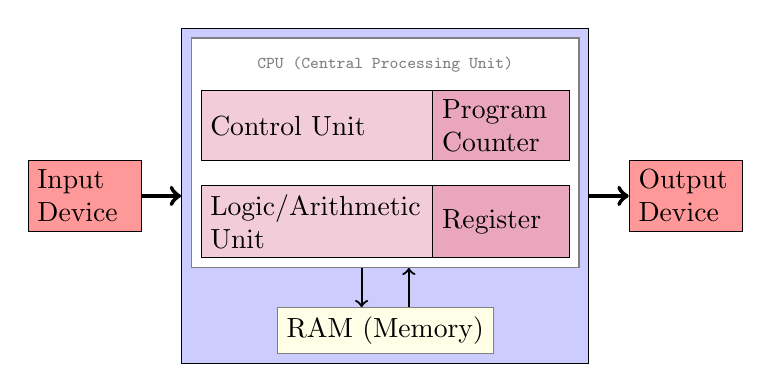
\begin{tikzpicture}[
  node distance=5mm,
  title/.style={font=\fontsize{6}{6}\color{black!50}\ttfamily}
  ]

  \begin{pgfonlayer}{main}
    \node (cputtl) [title] {CPU (Central Processing Unit) };

    \node (cu) [below=of cputtl,yshift=4mm,minimum height=7mm,
       rectangle split, rectangle split horizontal, rectangle split parts=2, draw,
       text centered,draw=black,line width=0.1mm,
       rectangle split part fill={purple!20,purple!35}]
       {\nodepart{one}\parbox{27mm}{Control Unit}
       \nodepart{two}\parbox{15mm}{Program Counter}};
    \node (lu) [below=of cu, yshift=2mm,minimum height=7mm,
       rectangle split, rectangle split horizontal, rectangle split parts=2, draw,
       text centered,draw=black,line width=0.1mm,
       rectangle split part fill={purple!20,purple!35}]
       {\nodepart{one}\parbox{27mm}{Logic/Arithmetic Unit}
       \nodepart{two}\parbox{15mm}{Register}};
  \end{pgfonlayer}

  \begin{pgfonlayer}{cpu}
    \node (cpu) [draw=black!50, fill=white, fit={(cputtl) (cu) (lu)}] {};
    \node (mem) [draw=black!50, fill=yellow!10, below=of cpu] {RAM (Memory)} ;
  \end{pgfonlayer}


  \begin{pgfonlayer}{background}
    \node (pc) [draw=black, fill=blue!20, fit={(cpu) (mem)}] {};
  \end{pgfonlayer}

  \begin{pgfonlayer}{main}
  \node (inp) [draw,fill=red!40,left=of pc] {\parbox{12mm}{Input Device}} ;
  \node (out) [draw,fill=red!40,right=of pc] {\parbox{12mm}{Output Device}} ;
  \path [draw,ultra thick,->] (inp) -> (pc) ;
  \path [draw,ultra thick,<-] (out) -> (pc) ;
  \path [draw,thick,<-] ([xshift=3mm]cpu.south) -> ([xshift=3mm]mem.north) ;
  \path [draw,thick,->] ([xshift=-3mm]cpu.south) -> ([xshift=-3mm]mem.north) ;
  \end{pgfonlayer}
\end{tikzpicture}
\end{document}

